\chapter{Теоретическая часть}
\label{cha:ch_1}

\section{Звук}
Звук - это вибрация, которая распространяется через воздух (или воду).
Например, при прослушивании музыки с компьютера колонки производят вибрации,
которые распространяются по воздуху, пока не достигнут уха человека.

Вибрации можно смоделировать с помощью синусоидальных волн.

\subsection{Чистый тон}
Чистый тон - это тон синусоидальной формы волны. Характеристики синусоиды:
\begin{itemize}
    \item Частота: количество циклов в секунду. Единица измерения - Герц (Гц), например, 100 Гц = 100 циклов в секунду.
    \item Амплитуда (связана с громкостью звука): размер каждого цикла.
\end{itemize}

Эти характеристики расшифровываются человеческим ухом для формирования звука.
Человек может слышать чистые тоны от $20$ Гц до $20 000$ Гц,
и этот диапазон уменьшается с возрастом. Для сравнения, свет, который видит человек,
состоит из синусоид от $4 * 10^{14}$ Гц до $7.9 * 10^{14}$ Гц.

Человеческое восприятие громкости зависит от частоты чистого тона.
Например, чистый тон с амплитудой равной $10$ и частотой $30$ Гц будет тише,
чем чистый тон с амплитудой $10$ и частотой $1000$ Гц.
Человеческие уши воспринимают звук в соответствии с психоакустической моделью.

Чистых тонов в природе не существует, однако каждый звук в мире - это сумма
нескольких чистых тонов с разными амплитудами.

\subsection{Музыкальные ноты}
Ноты разделены на октавы. В большинстве западных стран октава представляет
собой набор из 8 нот (A, B, C, D, E, F, G в большинстве англоязычных
стран) со следующим свойством:
\begin{itemize}
    \item Частота ноты в октаве удваивается в следующей октаве.
    Например, частота А4 (А в 4-й октаве) на частоте 440 Гц в 2 раза
    превышает частоту А3 (А в 3-й октаве) на 220 Гц и в 4 раза больше
    частоты А2 (А во 2-й октаве) на 110 Гц.
\end{itemize}

% Для 4-й октавы ноты имеют следующую частоту:
% \begin{itemize}
%     \item C4 = 261.63 Гц
%     \item D4  = 293.67 Гц
%     \item E4 = 329.63 Гц
%     \item F4 = 349.23 Гц
%     \item G4 = 392 Гц
%     \item A4 = 440 Гц
%     \item B4 = 493.88 Гц
% \end{itemize}

Частотная чувствительность ушей логарифмическая. Это означает, что:
\begin{itemize}
    \item между 32.70 Гц и 61.74 Гц (1-я октава)
    \item или между 261.63 Гц и 466.16 Гц (4-я октава)
    \item или между 2 093 Гц и 3 951.07 Гц (7-я октава)
\end{itemize}

Человеческие уши распознают одинаковое количество нот.

\subsection{Тембр}
Одна и та же нота может звучать по-разному, если ее играют гитара, пианино или скрипка.
Причина в том, что у каждого инструмента свой тембр для данной ноты.

Для каждого инструмента воспроизводимый звук представляет собой множество частот,
которые звучат как данная нота (научный термин для музыкальной ноты - высота звука).
Этот звук имеет основную частоту (самая низкая частота) и несколько обертонов (любая частота выше основной).

Большинство инструментов производят гармоничные звуки.
Для этих инструментов обертоны являются кратными основной частоты и называются гармониками.
Например, композиция чистых тонов A2 (основной), A4 и A6 является гармонической,
тогда как композиция чистых тонов A2, B3, F5 является негармоничной.

Многие ударные инструменты (например, тарелки или барабаны) создают негармоничные звуки.

Примечание: высота звука (воспринимаемая музыкальная нота) может отсутствовать в звуке,
воспроизводимом инструментом. Например, если инструмент воспроизводит звук с чистыми
тонами A4, A6 и A8, человеческий мозг интерпретирует полученный звук как ноту A2.
Эта нота / высота звука будет A2, тогда как самая низкая частота звука - A4
(этот факт называется отсутствующим основным).

\subsection{Цифровое представление звука}
Чтобы хранить и проигрывать звук на электронных устройствах, его нужно оцифровать.

\subsubsection{Семплирование}
Аналоговые сигналы - это непрерывные сигналы, что означает, что если взять одну секунду
аналогового сигнала, то ее можно разделить на части, которые длятся доли секунды.
В цифровом мире нельзя позволить себе хранить бесконечное количество информации.
Нужно иметь минимальную единицу времени, например, 1 миллисекунду.
В течение этого промежутка времени звук не сможет измениться, поэтому этот промежуток должен быть
достаточно коротким, чтобы цифровой сигнал звучал как аналоговый, и достаточно большой,
чтобы ограничить пространство, необходимое для хранения.

Эта задача называется семплированием.
\begin{figure}[H]
    \begin{center}
        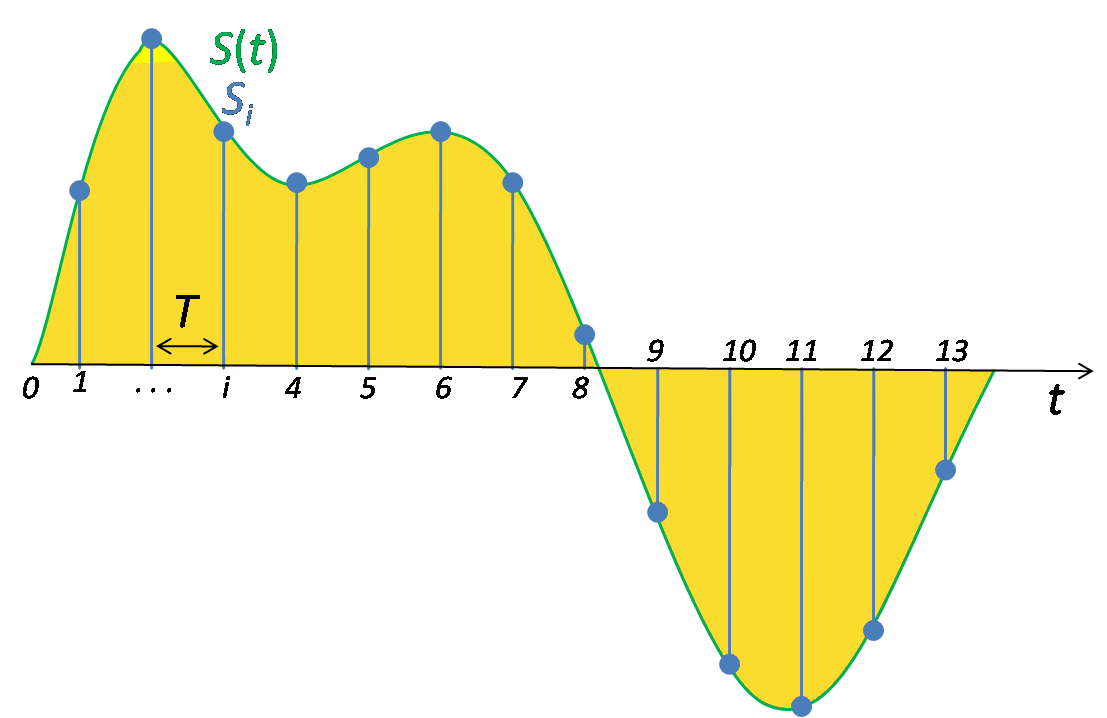
\includegraphics[scale=0.3]{inc/img/Signal_Sampling.png}
        \caption{Пример семплирования}
    \end{center}
\end{figure}

Стандартная единица времени в цифровой музыке составляет 44100 единиц (или сэмплов) в секунду.
Эта величина выбрана в связи с теоремой Котельникова, из которой следует,
что для оцифровки синусоиды частоты $F$ требуется, по меньшей мере, 2 точки на цикл.
Так как человек слышит в пределах 20 кГц, то соответственно для оцифровки сигналов нужно использовать
вдвое больше точек.

\subsubsection{Квантизация}
Громкость измеряет разницу между самым
низким и самым высоким уровнем звука в песне.
Как и в случае с семплированием, для оцифровки сигнала требуется иметь ограниченное количество
уровней громкости.

Эта задача называется квантизацией.
\begin{figure}[H]
    \begin{center}
        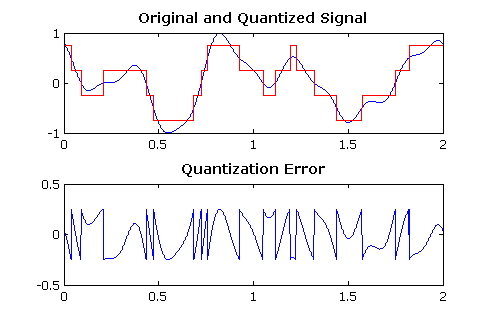
\includegraphics[scale=0.7]{inc/img/Quanterr.png}
        \caption{Пример квантизации}
    \end{center}
\end{figure}

\subsection{Спектрограмма}
Музыкальное произведение исполняется несколькими инструментами и певцами.
Все эти инструменты производят комбинацию синусоидальных волн на нескольких частотах,
и в целом комбинация синусоидальных волн еще больше.

Можно визуализировать музыку с помощью спектрограммы.
В большинстве случаев спектрограмма представляет собой трехмерный график, где:
\begin{itemize}
    \item по оси X представлено время (точнее его промежуток),
    \item по оси Y представлена частота чистого тона
    \item третье измерение описывается цветом и соответствует амплитуде частоты в определенное время.
\end{itemize}

\begin{figure}[H]
    \begin{center}
        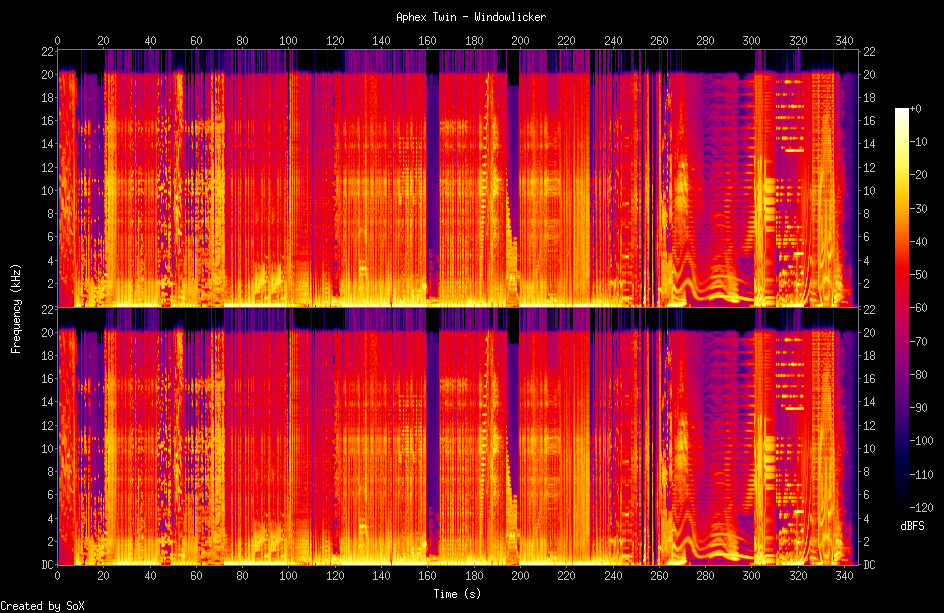
\includegraphics[scale=0.4]{inc/img/windowlicker.png}
        \caption{Спектрограмма Aphex Twin -- Windowlicker}
    \end{center}
\end{figure}

\subsection{Дискретное преобразование Фурье}
Для того, чтобы вычислить спектрограмму дискретного сигнала, нужно найти
его частоты. Это можно сделать с помощью дискретного преобразования Фурье (ДПФ).
ДПФ применяется к дискретным сигналам и его результатом является дискретный спектр (частоты внутри сигнала).

Формула ДПФ:
$$X(n) = \sum_{k=0}^{N-1} x(k) \times e^{-i \frac{2 \pi n k}{N}}$$,
где $N$ -- размер окна (количество семплов),
$X(n)$ -- $n$-ый диапазон частот,
$x(k)$ -- $k$-ый семпл сигнала

\section{Техника акустического отпечатка}
Для того, чтобы эффективно хранить и искать аудиофайлы, нужно
найти какое-нибудь компактное представление, которое при этом будет
максимально правдоподобно их описывать.
Это представление называется акустическим отпечатком (фингерпринтом) аудиофайла.
Существует множество видов таких отпечатков, но большинство методов
находят представление аудиофайлов в виде вектора хешей.

Факторы эффективности:
\begin{enumerate}[label=\arabic*.]
    \item Хеши максимизируют произведение функций энтропии и точности:
    \begin{figure}[H]
        \begin{center}
            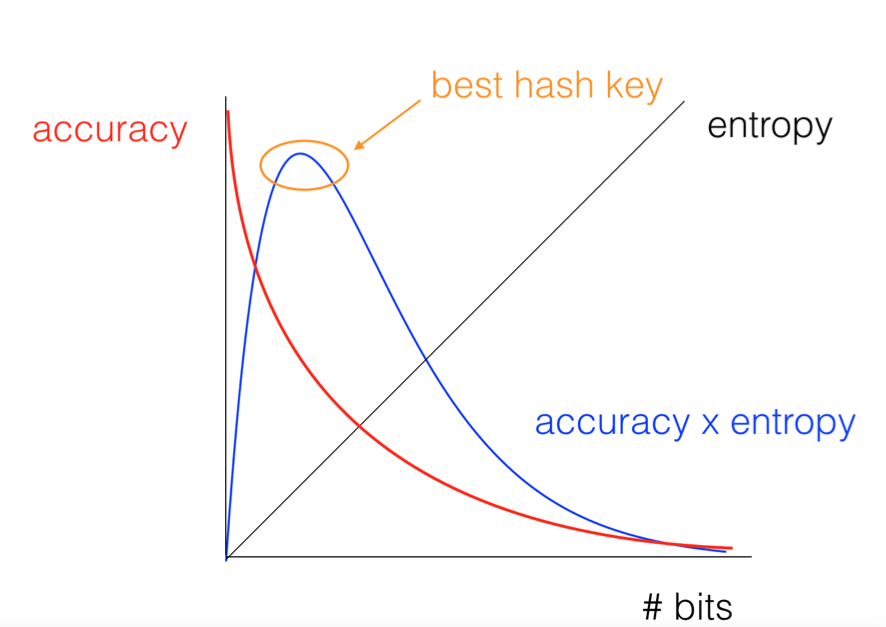
\includegraphics[scale=0.6]{inc/img/best_hp.png}
            \caption{Зависимость эффективности от точности и энтропии}
        \end{center}
    \end{figure}
    \item Биты хешей сбалансированы, декоррелированы и имеют высокую дисперсию
\end{enumerate}

\subsection{Общая идея}
Многие алгоритмы фингерпринтинга выглядят так:
\begin{enumerate}[label=\arabic*.]
    % \item Индексация:
    % \begin{enumerate}
        \item Посчитать спектрограмму аудиофайла
        \item Применить на ней какую-либо оконную функцию (спектрально-временные фильтры)
        \item Конвертировать результат в вектор хешей
    %     \item Посчитать обратный индекс вида:
    %     $$hash \to [... \{song\_id,\ offset\} ... ]$$, где $offset$ -- это
    %     номер временного диапазона аудиофайла, соответствующего $song\_id$,
    %     в котором встречается $hash$.
    % \end{enumerate}
    % \item Поиск:
    % \begin{enumerate}
    %     \item Посчитать акустический отпечаток запроса
    %     \item Поскольку
    % \end{enumerate}
\end{enumerate}

\section{Метод хешпринтов}
Этот метод предложен в \cite{tsai}. Он, как и многие другие, находит представление
аудиофайла в виде вектора хешей.

Метод отличается следующими характеристиками:
\begin{enumerate}[label=\arabic*.]
    \item Обучение без учителя
    \item Высокая адаптивность к данным
    \item Независимость от силы сигнала (громкости звука)
\end{enumerate}

Самой важной отличительной чертой метода является обучение без учителя.
Такие методы, как, например, Chromaprint, описанный в \cite{chromaprint}, используют
заранее подготовленные спектрально-временные фильтры.
Метод хешпринтов находит эти фильтры непосредственно при индексации, что позволяет
ему учитывать специфику данных.
\begin{figure}[H]
    \begin{center}
        
\includegraphics[scale=0.3]{inc/img/chroma.png}
        \caption{Фильтры, используемые Chromaprint}
    \end{center}
\end{figure}

\subsection{Алгоритм вычисления хешпринта}
Для вычисления хешпринта, содержащего $N$ бит, нужно проделать следующее:
\begin{enumerate}[label=\arabic*.]
    \item Посчитать спектрограмму.\\
    Результат этапа: матрица $Spectrogram \in \mathbb{R}^{B \times n}$, где $B$ -- количество частотных диапазонов,
    \begin{figure}[H]
        \begin{center}
            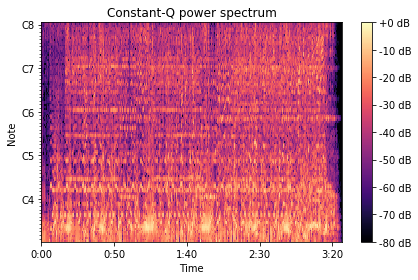
\includegraphics[scale=0.6]{inc/img/spectrogram.png}
            \caption{Спектрограмма}
        \end{center}
    \end{figure}
    $n$ -- количество временных диапазонов.
    \item Собрать контекстные фреймы полученной спектрограммы.
    Фреймы рассчитываются следующим образом:
    $$frame_i = V_{i-w}...V_{i+w}$$, где $V_i$ -- столбец спектрограммы, $w$ -- количество столбцов контекста.\\
    Результат этапа: матрица $Frames \in \mathbb{R}^{Bw \times n}$
    \begin{figure}[H]
        \begin{center}
            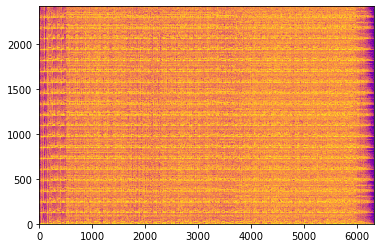
\includegraphics[scale=0.6]{inc/img/frame.png}
            \caption{Матрица фреймов}
        \end{center}
    \end{figure}
    \item Применить к фреймам спектрально-временные фильтры. Фильтры представляют собой
    $N \times Bw$ матрицу и расситываются c помощью алгоритма обучения без учителя
    путем решения задачи оптимизации.\\
    Результат этапа: матрица признаков $Features \in \mathbb{R}^{N \times n}$.
    \begin{figure}[H]
        \begin{minipage}{.5\textwidth}
            \centering
            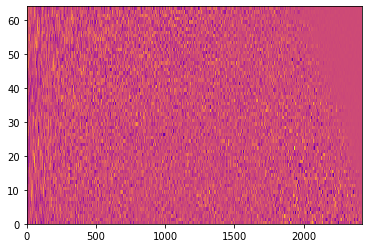
\includegraphics[scale=0.6]{inc/img/filters.png}
            \caption{Фильтры}
        \end{minipage}%
        \begin{minipage}{.5\textwidth}
            \centering
            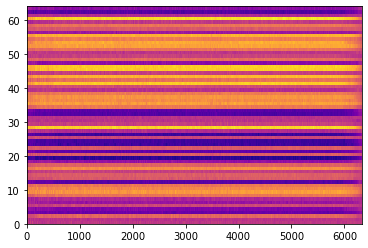
\includegraphics[scale=0.6]{inc/img/features.png}
            \caption{Матрица признаков}
        \end{minipage}
    \end{figure}
    \item Посчитать дельту -- изменение признаков в течение промежутка $T$.
    Дельта рассчитывается по формуле:
    $$\Delta_i = feature_i - feature_{i+T}$$
    \begin{figure}[H]
        \begin{center}
            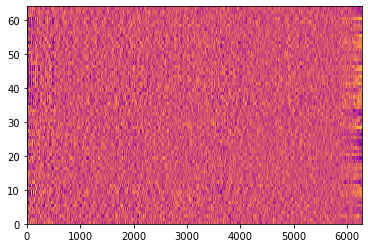
\includegraphics[scale=0.6]{inc/img/delta.png}
            \caption{Дельта}
        \end{center}
    \end{figure}
    \item Наложить функцию порога и упаковать результат в хешпринты:
    $$hashprint_i = intN(\Delta_i > 0)$$
    \begin{figure}[H]
        \begin{center}
            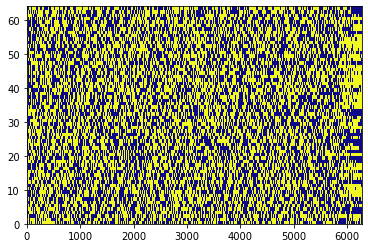
\includegraphics[scale=0.6]{inc/img/thres.png}
            \caption{Результат наложения функции порога}
        \end{center}
    \end{figure}
\end{enumerate}

\subsection{Вычисление спектрально-временных фильтров}
Фильтры подбираются таким образом, чтобы признаки, полученные при их наложении,
имели максимальную дисперсию и в то же время были декоррелированы.\\
Для этого можно применить метод главных компонент (PCA):
\begin{enumerate}[label=\arabic*.]
    \item Посчитать ковариационные матрицы для всех матриц фреймов в базе
    и просуммировать их.\\
    Результат этапа: матрица $CovarianceMatrix \in \mathbb{R}^{Bw \times Bw}$
    \item Найти $N$ собственных векторов с максимальными собственными значениями.\\
    Результат этапа: матрица $Filters \in \mathbb{R}^{N \times Bw}$
\end{enumerate}

\section{Задача идентификации живых отрывков}
Поскольку речь идет о нечетком поиске, то мы хотим учесть как можно
больше нюансов (признаков) сигнала. Поэтому будем представлять аудиофайлы в виде
64-битных хешпринтов. Также в качестве спектрограммы возьмем CQT спектрограмму -
она хороша тем, что ее частотные диапазоны подобраны таким образом, что они
соответствуют конкретным нотам.

\subsection{Хранение и поиск}
У живого исполнения с большой долей вероятности будет много общих признаков
в определенные моменты времени со студийным оригиналом. Также мы знаем, что
если какой-то аудиофайл является отрывком другого, то это значит что существует
такой отступ $offset$, что $fragment \approx original[offset..]$.

Таким образом, задача обретает вид:
$$ans = \argmin_{original, offset}d(fragment, original[offset..])$$,
где $d$ -- некоторая метрика. Проще говоря, мы хотим минимизировать расстояние между
отрывком и студийным оригиналом. Также стоит отметить, что такой подход подразумевает,
что музыкант не сильно изменил темп исполнения по сравнению с оригиналом.

\subsection{Почему обратный индекс не подходит}
Хранение и поиск аудиофайлов можно было бы организовать следующим образом:
\begin{enumerate}[label=\arabic*.]
    \item Построим обратный индекс вида:
    $$hashprint \to [...\{song\_id, offset\}...]$$
    \item Заводим счетчик. Для каждого хешпринта отрывка
    найдем все пары $\{song\_id, offset\}$, в которых содержатся
    соответствующие хешпринты и увеличим для них счетчик.
    \item Возвращаем пару с максимальным значением счетчика.
\end{enumerate}
У такого подхода есть одна проблема. Мы имеем дело с пространством довольно
большой размерности и вероятность того, что в отрывке и оригинале в один момент времени
встретятся полностью одинаковые хешпринты очень мала.

\subsection{Вариант авторов метода}
В качестве метрики берется сумма расстояний Хемминга между соответствующими хешпринтами
при прикладывании отрывка к оригиналу.
Также подразумевается, что есть некий сервис, который по GPS определит
ближайший концерт и соответственно исполнителя, что позволит проверить лишь малую часть базы.\\
Сам же поиск выглядит так:
\begin{enumerate}[label=\arabic*.]
    \item Для каждого оригинала из базы: прикладываем к нему отрывок и ищем такой отступ, чтобы сумма расстояний
    Хемминга между соответствующими хешпринтами была минимальной.
    \begin{figure}[H]
        \begin{center}
            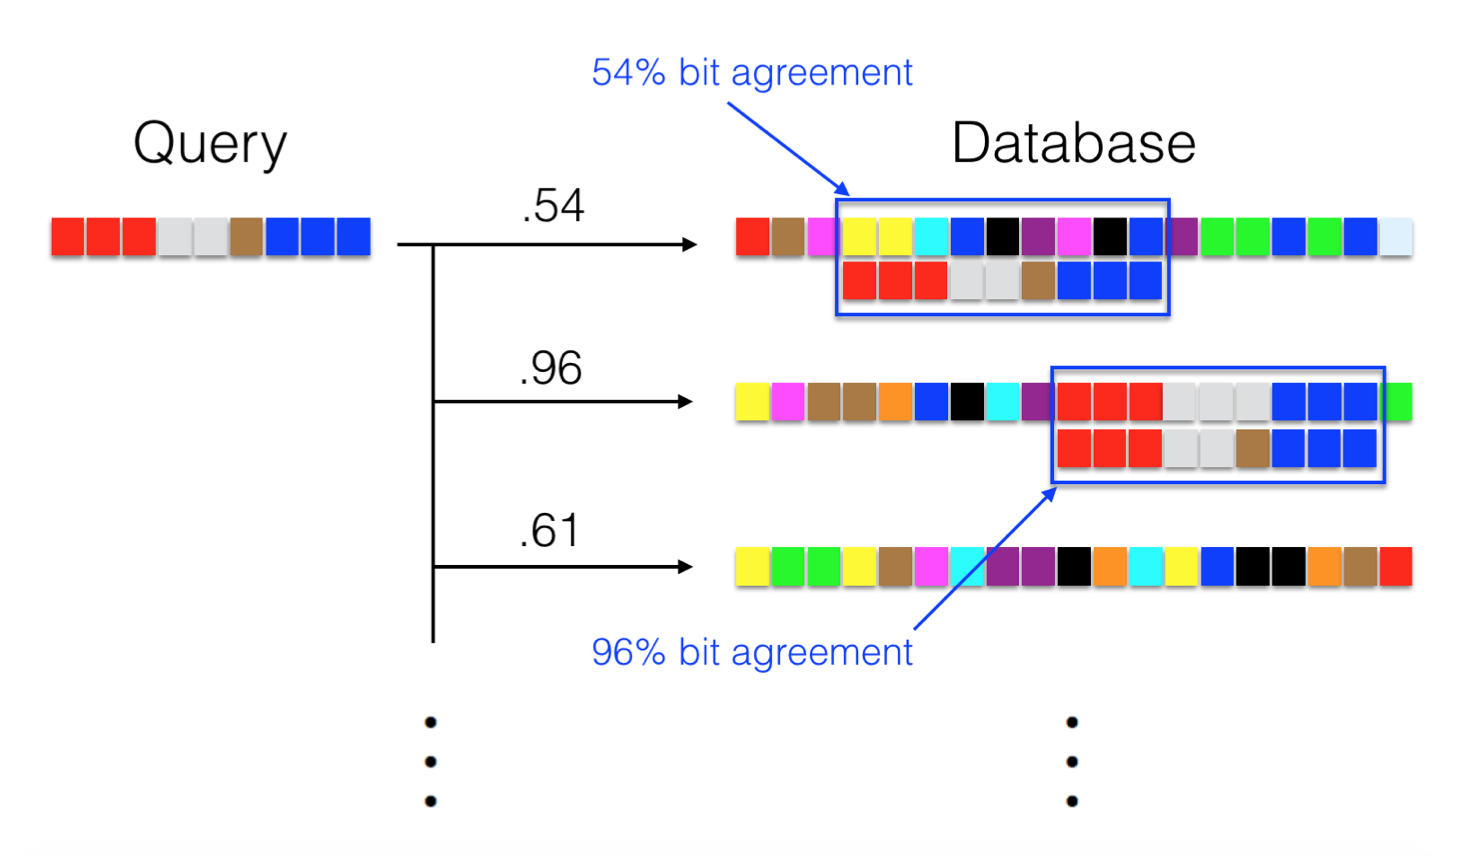
\includegraphics[scale=0.5]{inc/img/query.png}
            \caption{Пример обработки запроса}
        \end{center}
    \end{figure}
    \item Собираем результаты, сортируем и возвращаем top-N.
\end{enumerate}

Минус такого подхода -- GPS сервис:
\begin{enumerate}[label=\arabic*.]
    \item Точка отказа. Упадет сервис -- упадет вся система
    \item Затраты на разработку и поддержку сервиса
    \item Если это внешний сервис, то первый пункт становится еще большей проблемой
\end{enumerate}

Конечно, чаще всего человек знает на чей концерт он пришел и нужды в GPS сервисе не будет.
С другой стороны в наше время наблюдается рост числа музыкантов (по крайней мере в России),
поскольку делать музыку и делиться ей стало легче чем когда-либо.
Многие из этих музыкантов неизвестны широкому кругу слушателей, и они не готовы тратить
деньги на рекламу своего творчества, но периодически выступают на различных концертах
и фестивалях, где публика их возможно не узнает.

Но главная проблема в том, что этот метод имеет большой потенциал для применения
в других областях (например, классификация ЭКГ), в которых GPS сервис никак не поможет.
Чтобы сократить время поиска, нужно научиться каким-то образом отсекать большую часть данных.

\subsection{Метод k-ближайших соседей}
Можно взять вариант поиска с обратным индексом и заменить обратный индекс на
поиск k-ближайших соседей. Нам не критично, чтобы находились абсолютно все ближайшие соседи,
поэтому можно использовать методы приближенного поиска ближайших соседей
(approximate nearest neighbor), у которых выше производительность.

Мною было рассмотрено два алгоритма:
\begin{itemize}
    \item Метод случайных проекций.
    \item Иерархический маленький мир (HNSW)
\end{itemize}

Лучше всего себя показал HNSW.

\subsubsection{Метод случайных проекций}
Разбивает пространство гиперплоскостями и строит несколько бинарных деревьев.
Реализация: \href{https://github.com/spotify/annoy}{annoy}
\begin{itemize}
    \item[$-$] Производительность хуже, чем у другого алгоритма
    \item[$-$] Требует много памяти
\end{itemize}

\begin{figure}[H]
    \centering
    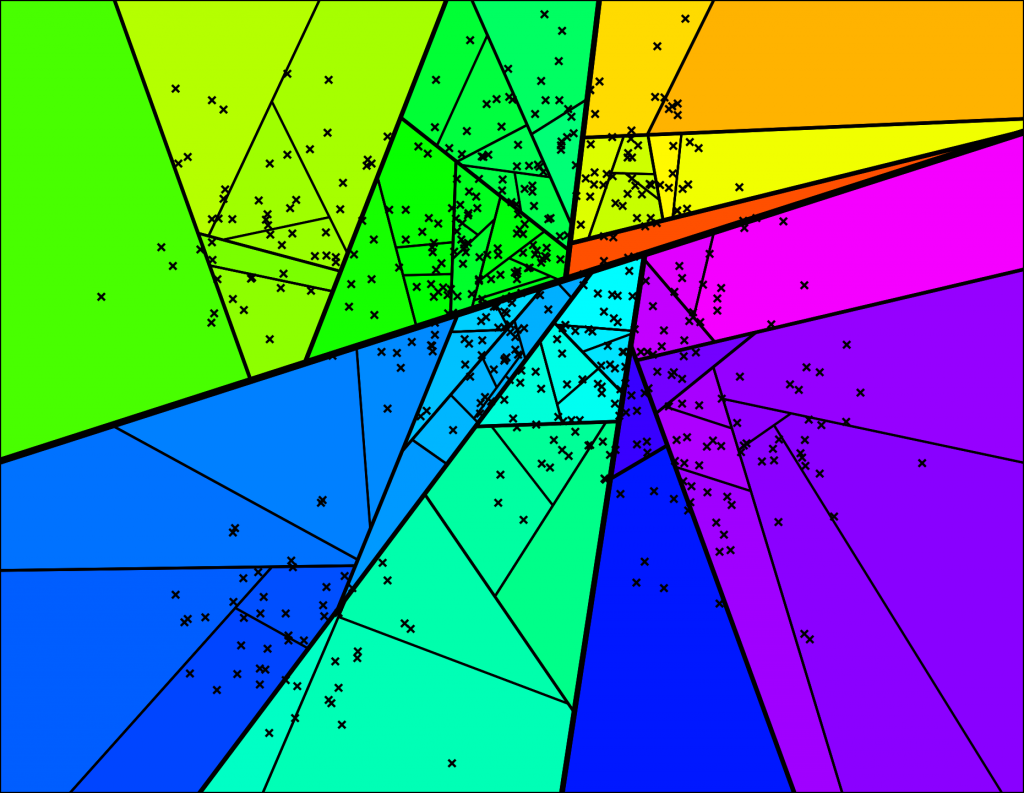
\includegraphics[scale=0.5]{inc/img/annspace.png}
    \caption{Пространство, разбитое гиперплоскостями}
\end{figure}

\begin{figure}[H]
    \centering
    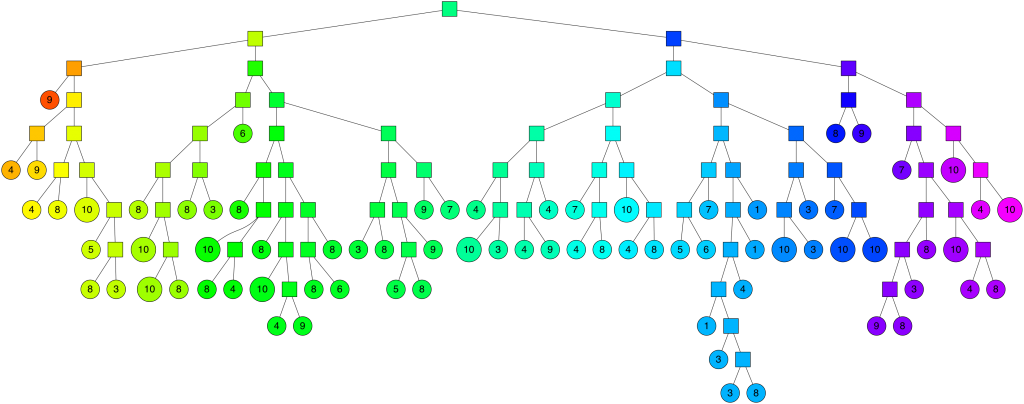
\includegraphics[scale=0.57]{inc/img/anntree.png}
    \caption{Соответствующее разбиению бинарное дерево}
\end{figure}

\subsubsection{Иерархический маленький мир}
Граф <<мир тесен>> -- это такой граф, в котором типичное расстояние $L$ между двумя
произвольно выбранными вершинами растёт пропорционально логарифму от числа
вершин: $L \propto \log{N}$.

В библиотеке \href{https://github.com/nmslib/nmslib}{nmslib} реализован алгоритм HNSW,
описанный в \cite{hnsw}. HNSW совмещает в себе свойства графа <<мир тесен>> и списка с пропусками.
По сути это иерархия графов, которая состоит из $n$ слоев: на нулевом слое представлены
все объекты, а по мере увеличения слоя -- все меньшая и меньшая их подвыборка.
При этом все объекты на слое $n+1$ есть и на слое $n$.
\begin{figure}[H]
    \begin{center}
        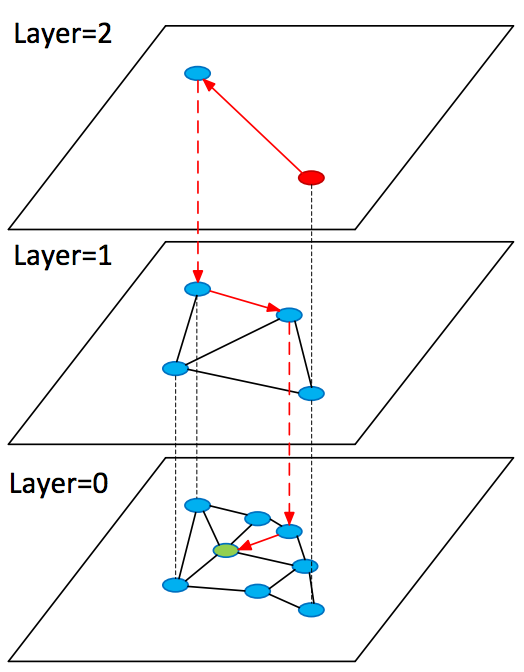
\includegraphics[scale=0.4]{inc/img/hnsw.png}
        \caption{Пример графа}
    \end{center}
\end{figure}

При поиске старт происходит со случайной вершины в графе верхнего слоя, там мы быстро
находим близкие к запросу вершины и возобновляем поиск с них на предыдущем слое.


Алгоритм очень легко масштабируется -- можно сделать ребро между вершинами, находящимися
на разных физических машинах. Также у HNSW хорошая производительность и небольшие затраты
на память.